\begin{figure}[ht!]
    \begin{subfigure}{\linewidth}
        %\caption{}
        \centering
        % include first image
        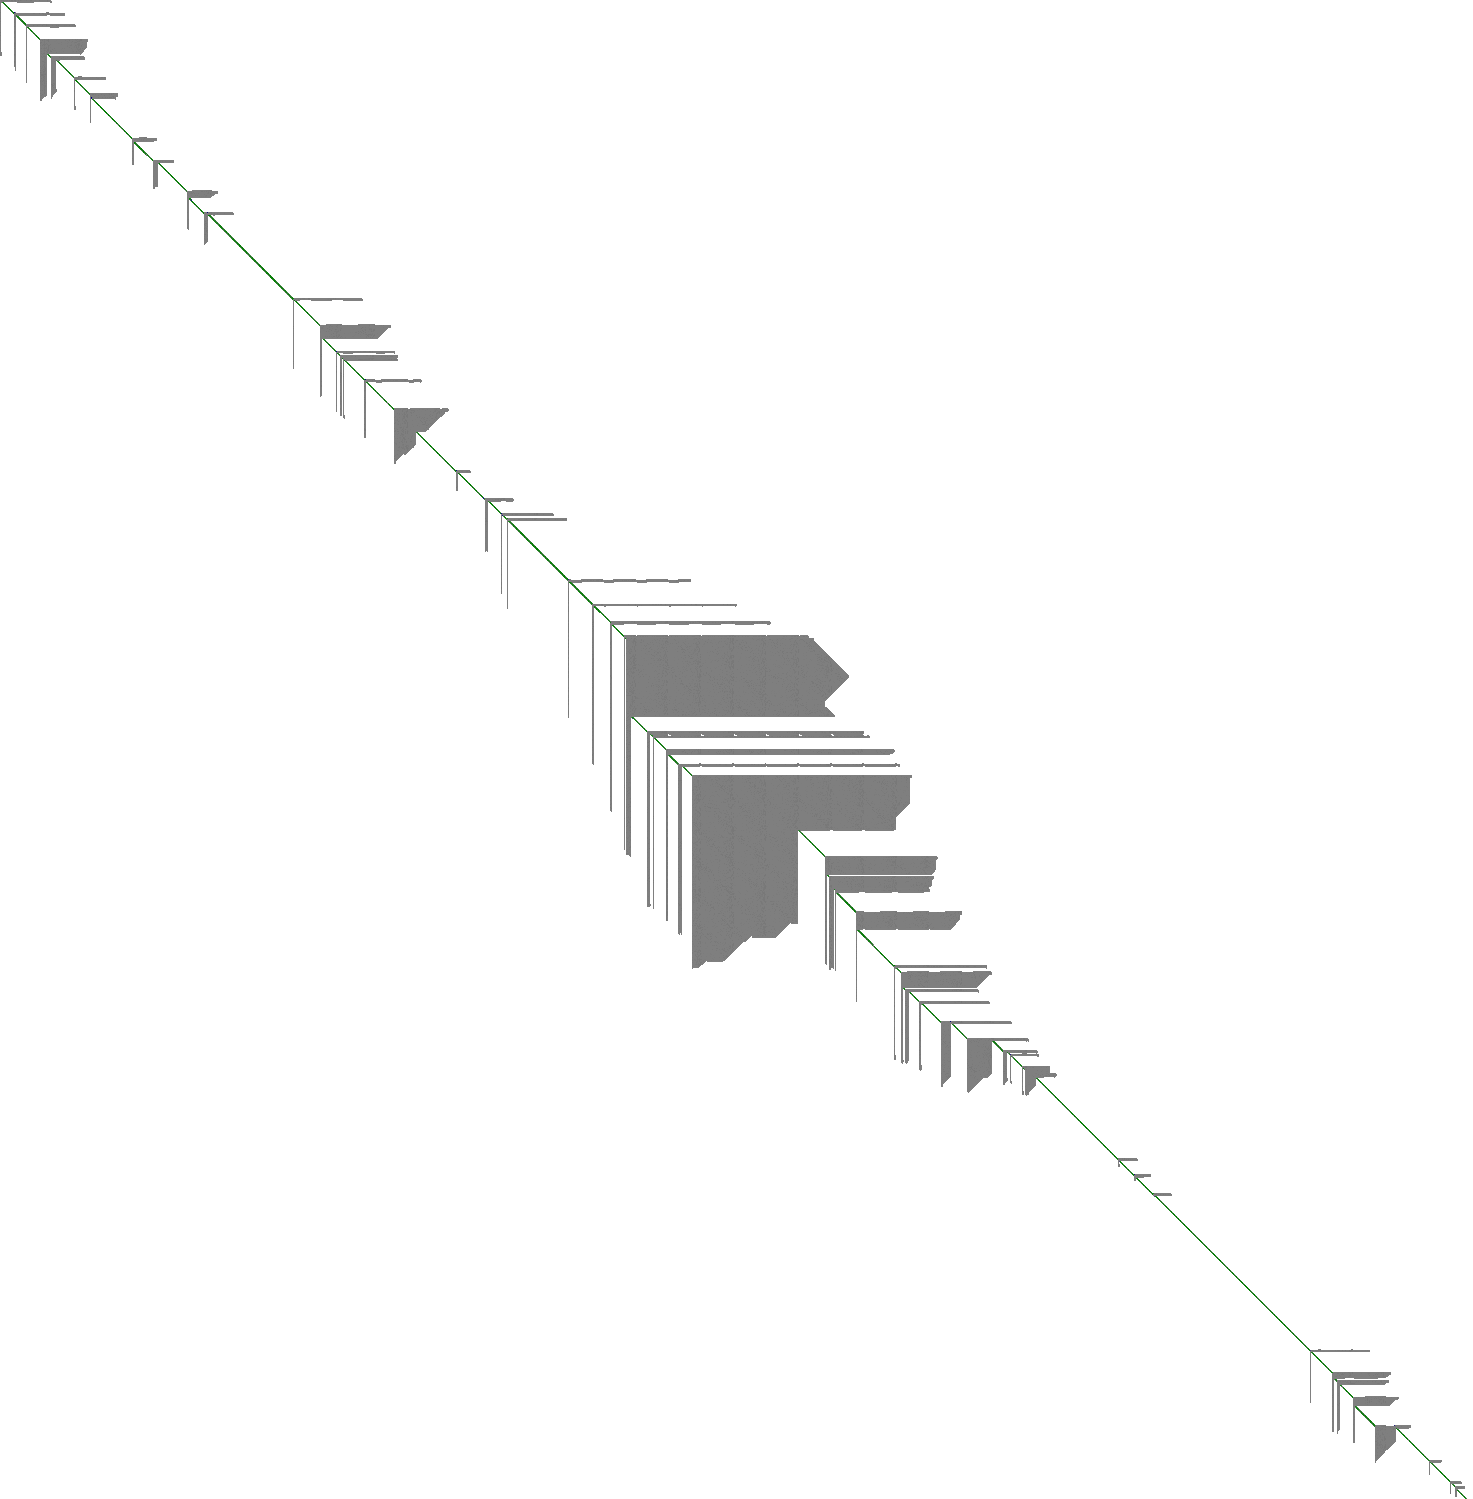
\includegraphics[width=1.0\linewidth, trim=-0cm 2cm 0 0cm]{fig/wflign.png}
        \label{fig:bad-sorting}
    \end{subfigure}
%	\includegraphics[width=\linewidth]{fig/metrics/chr4.pan.HTTex1.gfa.multiqc_odgi_stats.png}
    \caption{
      \textit{wflign} exploration of the alignment of $\sim$560kbp homologus segments of two \textit{Escherichia coli} genomes (GenBank NC\_000913.3 and NC\_008563.1).
      Gray indicates cells explored by WF$\lambda$.
      Blue cells are attempted, failed local WFA alignments, while green cells indicate alignments that match the maximum local alignment score.
      %The traceback (not shown) drives through the 
    }
    \label{fig:wflambda}
\end{figure}
